\chapter{}\label{chap3}%%% 3

This\pageoriginale chapter is devoted to the following problem: given a discrete\break
group $G$ acting properly on a topological space, determine a
presentation of $G$ (by generators and relations) and if possible a
finite one. The treatment given here is due to Behr \cite{key1}, \cite{key2}. The
classical presentation of groups generated by reflections (Coxeter
\cite{key1}) is discussed in section \S\ \ref{chap3:sec3} by a similar method. 

\section[Finite presentations for discrete proper groups....]{Finite presentations for discrete proper groups\hfill\break of transformations}\label{chap3:sec1}%%% 1 

Let $G$ be a group operating on a connected topological space
$X$. Assume that each $s\in G$ acts continuously on $X$. Let $A
\subset X$ be such that  
\begin{enumerate}[(1)]
\item $GA = X$
\item $G(A | A) A$ is a neighbourhood of $A$.
\end{enumerate}

\begin{prop*}
  $S = G(A|A)$ generates $G$.
\end{prop*}

\begin{proof}
  Let $G'$ be the subgroup of $G$ generated by $S$. We first assert that
  $G'A = X$. In fact, it is clear that $G'A$ is open in $X$. $G'A$ is
  also closed in $X$. For, let $x = sa \in X, s \in G, a \in A$. Then $V
  = sSA$ is a neighbourhood of $x$. If $V \cap G'A \neq \not\phi$, we
  have $s \in G(G'A|SA) \subset G' G(A | A) S \subset G'$, so that $x \in
  G'A$. Since $X$ is connected, we have $G' A = X$, Now, let $a \in
  A$. For any $s \in G$, we have $s' \in G', a' \in A$ such that $sa =
  s' a'$. Hence $s^{-1} s' \in S \subset G'$. Hence $s \in G'$. 
\end{proof}

\begin{remark*} 
  If $G$ is a locally compact group operating on a
  space $X$, and $A \subset X$ has properties 1) and 2) above, and
  if further $G (A | A) = S$ is relatively\pageoriginale compact in $G$, then $G$
  \textit{acts properly} on $X$. In fact, for $x = sa, x' = s' a' (s, s'
  \in G, a, a' \in A), U = s SA$ and $U' = s' SA$ are respectively
  neighbourhoods of $x$ and $x'$, and we see easily that $G(U | U') = s
  S^3 s'^{-1}$. 
\end{remark*}

In particular, if $S$ is finite, we are in the case of a discrete group
acting property. 

\begin{lemma*}
  Let $G$ be a discrete group acting continuously on a connected
  topological space $X$. Let $A$ be a closed subset of $X$ such that  
  \begin{enumerate}[\rm(1)]
  \item $GA = X$, 
  \item for each $x \in A$, there exists a finite subset $S_x$ of
    $G(A|A)$ such that $S_xA$ is a neighbourhood of $x$, 
  \item $A$ is connected, 
  \item any connected covering of $X$ which admits a section over $A$
    is trivial.  
  \end{enumerate}
  
  Let $L(S)$ be the free group generated by $S = G(A|A)$; for each $s
  \in G$, let $s_L$ be the generator of $L(S)$ corresponding to
  $s$. Then $G$ is isomorphic to the quotient group $L(S)/_{K}$, where
  $K$ is the normal sub group to $L(S)$ generated by the elements $s_L
  s_L' s_L''$ with $s, s' , s'' \in S$ and $ss' s'' = e$. 
\end{lemma*}

\begin{proof}
  Let us set $G = L(S)/_{K}$. For $s \in S$, let $s \in G$ denote $s_L
  \mod K$, and let $S = \{ s | s \in S \}$. Then we have: 
  \begin{enumerate}[(i)]
  \item $e \in S$
  \item $S = (S)^{-1}$; in fact, for $s \in S$, $(s)^{-1} = (s^{-1})$;
  \item if $s, s' in S$ are such that $ss' \in S$, then $s s' \in S$;
    in fact $s s' = ss'$. 
  \end{enumerate}
\end{proof}

It\pageoriginale is clear that $\underbar{e} \in \underbar{S}$. Also, since
$S^{-1}=S$ (iii) implies (ii). To prove (iii) note that $
\underbar{s} \,\underbar{s}'(\underbar{s} \underbar{s}')^{-1}=
\underbar{e}$, since $s_L s'_L ((s s')^{-1}_L) \in K$. 

We put the discrete topology on $\underbar{G}$ and consider the
product space $\underbar{G} \times A$. Let $\varphi : \underbar{G} \to
G$ be the homomorphism induced by the mapping $s_L  \rightsquigarrow
s$; clearly, $\varphi$ is surjective. We define a relation
$\mathcal{R}$  on $\underbar{G} \times A$ by setting $(t,a)
\mathcal{R}(t', a')$ if $\varphi(t)a = \varphi(t')a'$ and $t^{-1}t' \in
\underbar{S}$. From (i), (ii) and (iii) above, it follows that
$\mathcal{R}$ is an equivalence relation on $\underbar{G} \times
A$. Let $Y$ be the quotient space $(G \times
\underbar{A})_{/\mathcal{R}}$, and $q: \underbar{G} \times A \to Y$ be
the natural mapping. The mapping $(t, a) \rightsquigarrow \varphi (t)$ a
of $\underbar{G} \times A$ into $X$ induces a mapping $f: Y \to X$. We
make $\underbar{G}$ act on $Y$ by setting $rq (t,a) = q(rt,a); r,t \in
\underbar{G}, a \in A. \underbar{G}$ also acts on $X$ through
$\varphi$, and it is clear that $f$ commutes with the action of
$\underbar{G}$. 

We now wish to prove that $f: Y \to X$ is a connected covering, with
$H=$ ker $\varphi$ as the group of covering transformations. We do
this in several steps. 
\begin{enumerate}[(i)]
\item \textit{ $f$ is surjective}. In fact, $f(Y) = \varphi
  (\underbar{G}) A = GA =X$. 
\item \textit{ $f$ is locally injective}. We remark first that $f$ is
  injective on $q(\underbar{S} \times A)$. In fact, let $s,s' \in S$
  and $f q(\underbar{s},a) = f q(\underbar{s'}, a')$. Then $sa = s'
  a'$, hence $s^{-1} s' \in S$, implying $\underbar{s}^{-1}
  \underbar{s}' \in \underbar{S}$. This means that $
  q(\underbar{s},a) =  q(\underbar{s'},a')$.  We shall prove now that
  $q(\underbar{S} \times A)$ is a neighbourhood of $q( \underbar{e}
  \times A)$. It will follow that $f$ is locally injective. 
  
  Let $B$= interior of $SA$; and for $s \in S$, let $B_s = A \cap
  (s^{-1} B)$. Clearly, $B=\bigcup \limits_{s \in S} s B_s$. Let $L =
  \bigcup \limits_{s \in S} (\underbar{s} \times B_s)$.  Clearly, $q
  (\underbar{S} \times A) \supset q(L) \supset q (\underbar{e} \times
  A)$.\pageoriginale We now assert that $q(L)$ is open in $Y$, i.e.,
  that $L' = q^{-1} 
  (q((L)$ is open $\underbar{G} \times A$. In fact let $(t,a) \in L'$. 
  
  Then, for some $b \in B_s, \varphi (t) a = sb$ and $t^{-1}
  \underbar{s} \in \underbar{S}$. Let $S'=\{  s' in S| sb \in s' A \}$,
  and $W = \bigcup\limits_{s' \in S'}  s'B_{s'}$. Then $W \supset B \cap
  \bigcup \limits_{s' \in S' \cap S_{sb}}s' A$, hence $W$ is a
  neighbourhood of sb in $X$. Then $\varphi(t^{-1})W$ is a
  neighbourhood of a in $X$, and it is easily seen that the
  neighbourhood $\{ t \} \times \{ A \cap \varphi (t^{-1}) W \}$ of
  $(t,a)$ is contained in $L'$. 

\item \textit{For every $x \in X$, there are local sections for $f$ at $x$}. 
  
  It is sufficient to give a section on $SA$. To each $ h \in H = \ker
  \varphi$, we associate the section $\sigma_h : SA \to Y$ defined by
  $sa\, \rightsquigarrow q(h \underbar{s},a). \sigma_h$ is well-defined: if
  $sa=s'a'~ s,s'$ in $(S; a,a' \in A) , s^{-1} s' \in S$, so that
  $q(h\underbar{s},a) =q(h \underbar{s}'a')$. Clearly,$f o \sigma_h$ =
  identity, and for every $s \in S, \sigma_h |sA$ is continuous. Since
  (2) holds, it follows that $\sigma_h$ is a section of $f$. 

\item $\underline{ f^{-1} (SA)} = \bigcup \limits_{h \in H}
  \underline{\sigma_h (SA)}$. In fact, let $f(q(t,a)) \in SA$.  
  
  Then $\varphi (t) a = sa'$ with $s \in S$ and $a' \in A$. Hence
  $\varphi(t^{-1}) s \in S$, i.e $t^{-1}h \underbar{s} \in
  \underbar{S}$ for suitable $h \in H$. Then clearly $\sigma_h
  (s,a')=q(t,a)$. 
\item \textit{If $h \neq h' \sigma_h (SA) \cap \sigma_h' (SA)= \phi
  $}. Suppose, for $h, h' \in H$, that $\sigma_h (s,a)=
  \sigma_{h'} (s', a')(s,s' \in S$ and $a, a' \in A)$; i.e., $q(h
  \underbar{s}, a) = q(h' \underbar{s}', a')$. We have then
  $\underbar{s}^{-1} h^{-1}h' \underbar{s}' = \underbar{s}''$, with $s''
  \in S$. 

  Hence $h^{-1} h' = \underbar{s} \underbar{s}''
  \underbar{s}'^{-1}$. Since $\varphi (h^{-1}h')=e=s s'' s'^{-1}$ in $G$,
  it follows that $h^{-1} h' =\underbar{e} $ in $\underbar{G}$. 

\item \textit{$Y$ is connected}.\pageoriginale In fact, since $\underbar{G} q
  (\underbar{e} \times A) =Y$, we have only to verify that connected
  component $Y_o$ of $Y$ which contains $q(\underbar{e} \times A) $ is
  $\underbar{G}$-stable. But this is clear, since, for any $s \in S,
  q(\underbar{e} \times A) \cap \underbar{s} q(\underbar{e} \times A)
  \neq \phi$, and $\underbar{S}$ generates $\underbar{G}$ 
\end{enumerate}

Thus $(Y,f)$ is a connected covering of $X$, with $H=$ kernel
$\varphi$ as the group of covering transformations. Since (4) holds
it follows that $H= (\underbar{e})$, and this proves the lemma. 

\setcounter{thm}{0}
\begin{thm}\label{chap3:thm1}%the 1
  Let $G$ be a discrete group, acting continuously on a connected
  topological space $X$. Suppose that there exists a connected subset
  $A$ of $X$ such that  
  \begin{enumerate}[\rm(1)]
  \item $GA =X$,
  \item $G(A|A)$ is finite,
  \item $G(A|A)A$ is a neighbourhood of $A$.
  \end{enumerate}
  
  Suppose further that there exists a compact subset $C$ of $X$ such
  that any connected covering of $X$ which admits a section over $C$ is
  trivial. Then $G$ is finitely presentable. 
\end{thm}

\begin{proof}
  We first remark that $A$ may be assumed to be closed. In fact we shall
  verify the conditions (2) to (3) for $\bar{A}$.  Now, we note that
  $\bar{A} \subset S^2 A;$ for, if $x = sa \in \bar{A} (s \in G, a \in
  A)$. the neighbourhood sSA of a meets $A$, hence $s \in S^2$. Hence
  $G(\bar{A}|\bar{A}) \cap S^5$, and so is finite. Also, $S^3A$ is clearly
  a neighbourhood of $S^2 A \supset \bar{A}$, hence $G(\bar{A}|\bar{A})A$
  is a neighbourhood of $\bar{A}$. 
\end{proof}

Let now $S = G(A|A)$. For every n, $S^n A$ satisfies conditions
(1), (2), (3) of the lemma. If $n$ is large enough, $S^nA \supset C$, 
and therefore satisfies condition (4). Hence there exists a finite
presentation of\pageoriginale $G$ with $G(S^nA|S^nA) \subset S^{2n+1}$ as set of
generators.
 
\setcounter{rem}{0}
\begin{rem}%rem 1
  For a locally simply connected space $X$,the existence of a compact
  set $C$ satisfying the condition of the theorem means that $\prod_1
  (X)$ is finitely generated. 
\end{rem}

\begin{rem}%rem 2
  Suppose that, in Theorem \ref{chap3:thm1}, we drop the assumption that $A$ is
  connected. We can still assert that $G$ is finitely presentable, if
  $X$ is locally connected. We may assume that $A$ satisfies conditions
  (1), (2) and (4) of the lemma. The space $Y$ constructed above need
  not now be connected, so that we will have to enlarge $K$ suitably. 
\end{rem}

We retain the notation of the proof of Theorem \ref{chap3:thm1}. Let
$B=$ interior of $SA$, and let $B_o$ be a connected component of
$B$. We first prove that  
\begin{equation*}
  X= \cup G(B_o | B_1) G (B_1| B_2) \ldots G(B_{n-1}|B_n)B_{n}, \tag{*}
\end{equation*}
where the union is over all finite sequences $B_1, \ldots , B_n$
connected components of $B$. In fact, since $X$ is locally connected,
the connected components of $B$ are open, hence the right side $X'$ of
$(*)$ is open in $X$. 

Now let $x$ be any point of $X$. Since $GB=X$, we have $x \in t B'$,
for $t \in G$ and some connected component $B'$ of
$B$. Now suppose the neighbourhood $tB'$ of $x$ meets $X'$, say  
$$
\displaylines{\hfill 
   t B' \cap \{ G(B_o |B_1) \cdots G(B_{n-1}|B_n)B_n \} \neq
  \phi. \hfill \cr 
  \hfill \text{Then} \hfill  t\in G(B_o|B_1) \cdots G(B_{n-1}|B_n)
  G(B_n|B'),\phantom{then then the}\hfill \cr
  \text{hence}\hfill  x \in G(B_o|B_1) \cdots G(B_{n-1}|B_n) G(B_n|B')
  B' \subset X'.\hfill } 
$$

Hence $X'$ is also closed\pageoriginale in $X$. Hence $X' = X$.

We also have:

\noindent
(**)\quad For any $B_1,B_2 \subset B$ and any $t \in G(B_1|B_2)$, there
exists a $\underbar{t} \in \underbar{G}$ such that $\underbar{t}
\sigma_e (B_2) \cap \sigma_{\underbar{e}} (B_1) \neq \phi$ 

This is clear since $\varphi$ is surjective, and $\underbar{G}$ is
transitive on the fibres of $f$.  

Now let $s \in S$. By $(*)$, there exist connected components $B_1,
\ldots , B_n$ of $B$ such that $s B_\circ \cap \{ G(B_\circ B_1) \ldots
G(B_{n-1} B_n) B_n \} \neq \phi$. We thus have $t_i \in G(B_{i-1}
B_i),i = 1, \ldots , n$, such that $t^{-1}_{n+1} = s^{-1} t_1 \cdots
t_n \in G(B_o B_n)$. For each $t_i , i = 1, \ldots , n+1$, we choose
$\underbar{t}_i \in \underbar{G}$ as in $(**)$, and consider the
normal subgroup $K'$, of $\underbar{G}$ generated by all the
$\underbar{s}^{-1}\underbar{t1} \cdots t_{\underbar{n} +1}, s \in
S$. Obviously, $K' \subset H$. Hence $f: Y \to X$ induces a mapping
$f': Y' =K'/Y \to X$ such that the diagram  
\[
\xymatrix{Y \ar[dd]_f \ar[rd]^g &\\ 
& Y' \ar[ld]^{f'}\\
X & 
}
\]
is commutative; here $g:Y \to Y'$ is the natural mapping. Clearly
$(Y',f')$ is a covering of $X$ and $\underbar{G}' = \underbar{G}_{/K}$
operates on $Y'$, transitively on the fibres of $f'$. We now assert
that $Y'$ is connected. In fact let $Y'_o$ (\resp $Y_o)$ denote the
connected component of $Y'$ (\resp $Y$) which 
contains $g \sigma_{\underbar{e}}(B_o)$ (\resp $\sigma_e(B_o))$. Since
$f'(Y'_o) = X$, we need only prove that $Y'_o$ is stable under
$\underbar{G}'$. For this again it is sufficient to check that for any
$\underbar{s} \in \underbar{S}$, we have a $\underbar{t} \in K'$ such
that $\underbar{s}^{-1} \sigma_{\underbar{e}} (B_o) \cap \underbar{t} Y_o \neq
\phi$. In fact, we can choose $\underbar{t} = \underbar{s}^{-1}
t_{\underbar{1}} \cdots t_{n+1} \in K'$. 

Since\pageoriginale $A$ satisfies condition (4), it follows that $H_{/ K'}$, the
group of covering transformations of $(Y',f)$, is trivial. Hence $G
\approx \underbar{G}/_{K}'$ is finitely presentable . 

\begin{rem}%rem 3
  Let $G$ be a discrete group, acting properly on a locally compact
  connected space $X$ such $G^{/X}$ is compact. If $\prod_1 (X)$ is
  finitely generated, then $G$ is finitely presentable. 
\end{rem}

In fact, we can find a compact subset $A$ of $X$ containing a set of
loops which generate $\prod_1 (X)$, such that $GA = X$, and this $A$
satisfies the conditions of Theorem \ref{chap3:thm1}. 

In particular, since connected Lie groups have finitely generated
fundamental groups, we see that, in a connected Lie group, any
discrete subgroup with compact quotient is finitely presentable. 

\section[Finite presentations for groups of automorphisms....]{Finite presentations for groups of automorphisms of
  graphs}\label{chap3:sec2}%sec 2 

For the next result, we need some elementary notions about graphs.

A \textit{ graph} is a set $X$ in which there is associated to each $
x \in X$ a subset $\sum (x)$ of $X$ such that (i) for every $x \in
X, x \in \sum (x)$, and (ii) for any $x,y \in X, x \in \sum (y)$
implies $y \in \sum(x)$. A graph $X$ is \textit{ finite at} $x \in X$
if $\sum (x)$ is finite. 

A \textit{ path} in a graph $X$ is a sequence $(a_o,a_1 ,\ldots ,
a_n)$ of elements of $X$ such that $a_{i+1} \in \sum (a_i) , 0 \leq i
\leq n-1; a_o$ and $a_n$ are respectively the \textit{initial} and
\textit{end points} of the path, and if $a_o = a_n$, the path is
called a \textit{loop at }$a_o$. A graph is said to be
\textit{connected} if any two of its points can be joined by a path. 

Consider\pageoriginale the operations which respectively associate to
any path $(a_o ,\ldots , a_n)$ in the graph the path $(a_o, ,\ldots , a_{i}, a_{i+1},
\ldots a_n)$ and the path $(a_o, ,\ldots , a_i, b, a_i , \ldots,a_n)$
with $b \in \sum(a_i)$. Two paths in a graph are \textit{homotopic} if
we can obtain one from the other by means of a finite number of the
above operations and their inverses. The product of paths is defined
in the usual way. 

A loop $(a_o ,\ldots , a_n =a_o)$ is said to be of \textit{length}
$\leq m$ if $a_i = a_{m-i}$ for $0 \leq i \leq \dfrac{n-m}{2}$. A
graph $X$ is of \textit{breadth} $\leq m$ if every loop in $X$ is
homotopic to a product of loops of length $\leq m$. 

Let $X$ and $Y$ be graphs. A \textit{homomorphism} $f: X \to Y$ is a
mapping such that for every $x \in X, f ( \sum (x)) \subset
\sum(f(x))$.

Let $Y$ be a connected graph. A homomorphism $f:X \to Y$ is a 
\textit{covering} if, for every $y \in Y$ and $y' \in \sum(y)$, and every
$x \in f^{-1}(y)$, there exists a unique $x' \in \sum(x)$ such that
$f(x') =y'$. If $f$ is a covering, it is easily seen that any path in
$Y$ can be lifted to a path in $X$ with any given initial point. 

If $X$ is connected, and $f: X \to Y$ is a covering such that every
lift of any loop in $Y$ is a loop in $X$, then $f$ is bijective. In
fact, it is sufficient to assume that for a point $y_o \in Y$ and an
$x_o \in f^{-1}(y_o)$, the lift through $x_o$ of any loop at $y_o$ in
$Y$ of length $\leq $ breadth $Y$ is a loop. 

\begin{thm}\label{chap3:thm2}%the 2
  Let $X$ be a connected graph of finite breadth, finite at each point.
  Let $G$ be a transitive group of automorphisms of $X$. If the isotropy
  group is finitely presentable, then $G$ is finitely presentable.\pageoriginale 
\end{thm}

\begin{proof}
  Let $x_o \in X$. For each $x \in \sum (x_o)$,choose an $s_x \in G$
  such that $s_x x_o =x$, and let $S = \{ s_x |x \in \sum(x_o)\}$. Since
  $X$ is finite  at $x_o, S$ is a finite set. 
\end{proof}

Let $L(S)$ be the free group on the set, and let $H= G(x_o)$. Let
$L(S) \mathbb{X} H$ be the free product of $L(S)$ and $H$. We have a
homomorphism 
$$
\psi : L (S) \sharp H \to G
$$
induced by the obvious maps of $L(S)$ and $H$ into $G$. Since $X$ is
connected, we have $\psi (L(S)) x_o =X$, and hence $G = \psi
(L(S))H$. In particular, $\psi$ is surjective. 

Let $T$ be a finite set of generators of $H$. Let $s \in S, t \in
T$. We have ts$x_o \in \sum(x_o)$. Hence there exists a unique $s' \in
S$ such that tsx$_o = s' x_o$. Clearly ${s'}^{-1}ts \in H$. Denoting by
$s_L$ the element of $L(S)$ corresponding to $s \in S$, we consider
the normal subgroup $K$ of $L(S) \sharp H$ generated by the (finitely
many)elements of the following type  
\begin{enumerate}[(i)]
\item $(s'_{L})^{-1} t (s_L). (s'^{-1}ts)^{-1}; s \in S, t \in T$
\item $(s_1)_L (s_2)_L \cdots (s_n)_L (s_1 s_2 \cdots s_n)^{-1}; s_1,
  \ldots s_n \in S ,s_1 s_2 \cdots s_n \in H , n \leq $ breadth of
  $X$. 
\end{enumerate}

Clearly $K \subset \ker \psi$, hence $\psi$ induces a homomorphism 
$$
\varphi : \underbar{G}= (L(S) \sharp H)_{/K} \to G.
$$

We\pageoriginale shall prove now that $\varphi$ is an isomorphism. Since $L(S)
\sharp H$ is finitely presentable, this will prove that $G$ is
finitely presentable. 

Let $\underbar{H}$ be the image of $H$ in $\underbar{G}$. Since, for
any $s \in S$ and $t \in T,K$ contains an element of the type
$(s'_L)^{-1} t(s_L)h$ with $h \in H$, we see that
$\underbar{S}\underbar{H} = \underbar{H}\underbar{S}$ where
$\underbar{S}$ is the image of the set $\{ s_L | s \in S \} $ in
$\underbar{G}$. Let $Y = \underbar{G}_{/\underbar{H}}$, and
$q:\underbar{G} \to \underbar{H} $ the natural mapping. The mapping
$\underbar{t} \rightsquigarrow \varphi(\underbar{t})x_o$ of
$\underbar{G}$ onto $X$ induces a mapping $f : Y \to X$,  and we have
commutative diagram  
\[
\xymatrix{\underbar{G} \ar[d]_q \ar[r]^\varphi & G \ar[d]\\
Y \ar[r]^f & X}
\]
where $G \to X$ is the mapping $s \rightsquigarrow sx_o. \underbar{G}$
acts on $Y$ (by left multiplication), and we have for any $\underbar{t}
\in \underbar{G}$ and $y \in Y , f(\underbar{t} y) = \varphi
(\underbar{t}) f(y)$. 

We define the structure of a graph on $Y$ as follows. Set $y_o = q
(\underbar{e})$, and for any $y = \underbar{t} y_o \in Y$, set $\sum
(y) = \underbar{t} \underbar{S} y_o$. We check first that $\sum (y)$
is well-defined. In fact, let $y = \underbar{t}' y_o$. Then
$\underbar{t}' = \underbar{t} \underbar{h}$, with $\underbar{y} \in
\underbar{H}$. Hence for any $\underbar{s} \in \underbar{S},
\underbar{t}' \underbar{s} y_o = \underbar{t} \underbar{h}
\underbar{s} y_o= \underbar{t}\underbar{s}' \underbar{h} y_o =
\underbar{t} \underbar{s}'y_o$, since $\underbar{H} \underbar{S} =
\underbar{S} \underbar{H}$. The verification that $y_1 \in \sum (y_2)$
implies $y_2 \in \sum(y_1)$ is similar. Since $S$ generates
$\underbar{G}$ modulo $\underbar{H}$ (i.e. $\underbar{G} = \cup
\underbar{S}^n \underbar{H})$, it is easily seen that $Y$  is a
\textit{connected} graph. Moreover, $f$ is a homomorphism of
graphs. 

We assert now that $f$ is a covering. To prove this it is enough to
lift paths starting at $x_o$. Let $y \in f^{-1}(x_o)$. If $y =
\underbar{t}y_o$, we\pageoriginale have $\varphi (\underbar{t}) x_o = \varphi
(\underbar{t}) f(y_o)= f(\underbar{t} y_o) = x_o$, hence
$\varphi(\underbar{t}) \in H$. Now let $sx_o \in \sum (x_o)$. Then
there exists a unique $s' \in S$ such that $\varphi (\underbar{t})
sx_o = s'x_o$, and $y' = \underbar{t} \underbar{s}' y_o \in \sum
(y_o)$ is clearly the unique lift of $sx_o$ in $\sum (y_o)$. 

We verify finally that the lift of any loop of the type $(x_o,s_1 x_o
, \ldots, s_1$ $s_2 \cdots s_n x_o)$ with $n \leq $ breadth of $X$ is a
\textit{ loop}at $y_o \in Y$. This will prove that the covering $Y \to
X$ is trivial, since every loop at $x_o$ is homotopic to a product of
loops of this type.  Now, it is clear that $(y_o,s_1 y_o , \ldots ,
s_1 s_2 \cdots s_n y_o)$ is a path at $y_o$ which lifts the above
loop. And since $s_1 s_2 \cdots s_n = e$, we have $\underbar{s}_1
\ldots \underbar{s}_n \in \underbar{H}$, i.e. this path is a loop. 

Hence it follows that $f$ is bijective. Suppose now that $\underbar{t}
\in \underbar{G}$, and $\varphi (\underbar{t}) =e$ in $G$. Then,
$f(\underbar{t} y_o) =\varphi(\underbar{t}) x_o =x_o$. Since $f$ is
bijective, we must have $\underbar{t} \in \underbar{H}$. However,
$\varphi | \underbar{H}$ being injective, this means that
$\underbar{t} = \underbar{e}$ in $\underbar{G}$, and hence is finitely
presented. 

\begin{remark*}
  It follows from Theorem \ref{chap3:thm2} that if a group $G$ admits of a left
  invariant graph structure which is (i) connected, (ii) finite at
  each point, and (iii) of finite breadth, then $G$ is finitely
  presentable. The converse is also true, i.e. any finitely presentable
  group admits of a left-invariant graph structure which satisfies
  conditions (i), (ii) and (iii). In fact let $G$ be a finitely
  presentable group, and let $S$ be a finite set of generators of $G$
  such that $e \in S$, and $S = S^{-1}$. We define a graph structure on
  $G$ by setting, for any $t \in G$, 
  $$
  \sum(t) = \{ t' \in G|t^{-1}t' \in S \}.
  $$
\end{remark*}

It\pageoriginale is easy to see that this defines a graph structure on
$G$ which is 
left-invariant, connected, and finite at each point. We shall now
prove that the breadth of this graph is finite. 

Let $L(S)$ be the free group on $S$; for $s \in S$, we denote be $s_L$
the corresponding generator of $L(S)$. Let $K$ be the kernel of the
natural mapping $L(S) \to G$. Since any loop at $e$ in $G$ can be
written in the form $(e,s_1, s_1s_2, \ldots s_n =e)$, we see that $K$
is naturally isomorphic to the group of homotopy classes of loops at
$e$. 

Now, since $G$ is finitely presentable, we have by a theorem of
Schre\-ier a finite subset $F$ of $K$ such that $K$ is the normal
closure of $F$ in 
$L(G)$. It follows easily that, if for each element of $F$ we choose a
representative loop at $e$, and 1 is an upper bound for the lengths
of these loops, our graph structure on $G$ has breadth $\leq 1$. 

\setcounter{rem}{1}
\begin{rem}%rem 2
  Let $G$ be a group which has a finitely presentable normal subgroup
  $N$ such that $G_{/N}$ is finitely presentable. Then $G$ is finitely
  presentable. In fact, by the above remark, there exists a $G$-invariant
  graph structure on $G_{/N}$  which is connected, finite at each point,
  and of finite breadth. Since $G$ acts transitively on $G_{/N}$  with
  isotropy group $N$ which is finitely presentable, it follows from
  Theorem \ref{chap3:thm2} that $G$ is finitely presentable. 
\end{rem}

As an application of Theorem \ref{chap3:thm2}, we shall prove the following

\begin{thm}[Behr \cite{key2}]\label{chap3:thm3}%%%% 3
For any finite set $P$ of primes,
the group\break $GL(n \mathbb{Z}[P^{-1}])$ is finitely presentable. 

Here\pageoriginale
$\mathbb{Z}[P^{-1}]$ is the subring of the rationals $\mathbb{Q}$
generated by $P^{-1} = \{ p^{-1 }| p \in P \}$. To prove Theorem \ref{chap3:thm3}
we need some preliminaries. 

For any prime $p$, let $\mathbb{Q}_p$ be the $p$-adic field,
$\mathbb{Z}_p \subset \mathbb{Q}_p$ the ring of p-adic integers. Let
$\mathcal{R}$ be the set of all lattices in $\mathbb{Q}^n_p$. (A
\textit{lattice} in $\mathbb{Q}^n_p$ is a $\mathbb{Z}_p$-submodule
generated by a basis of $\mathbb{Q}^n_p$). 

If we set, for $A, B \in \mathcal{R}$,
$$
d(A,B)= \inf \{ r \in \mathbb{Z}^+ | p^r A \subset B, p^r B \subset A \}
$$
$d$ is a metric on $\mathcal{R}$. We define a graph structure on
$\mathcal{R}$ by setting, for any $A \in \mathcal{R}, \sum (A) = \{ B
\in \mathcal{R}| d(A,B)\leq 1 \}$. 

$\mathcal{R}$ is finite at every point. In fact,$d(A,B) \leq 1$
implies that $pA \subset B \subset p^{-1} A$, and this can hold (for a
given $A \in \mathcal{R}$) only for finitely many $B$. Also, 
$\mathcal{R}$ is connected, in view of the following
\end{thm}


\begin{prop*}
 Given $A, B \in \mathcal{R}, A  \neq B $, there
exists a $ C \in \mathcal{R}$ such that: 
\begin{enumerate}[(i)]
\item $d(A,C) =1$, and $d(C,B) = d(A,B)-1$;

\item for any $ D \in \mathcal{R}$, we have 
  $$
  d(D,C) \leq \sup \{ d(D,A), d(D,B)\}.
  $$
\end{enumerate}
\end{prop*}

\begin{proof}
  Since $\mathbb{Z}_p$ is a principal ideal domain, there exists a basis
  $(a_1, \ldots , a_n)$ for $A$, and integers $r_1, \ldots , r_n$, such
  that $(p^{r_1} a_1, \ldots ,p^{r_n} a_n)$ is a basis for $B$; clearly
  we have then $d(A,B) = \sup |r_i|$. Let $c_i =p_i^{\alpha(i)} a_i$, where  
  \begin{equation*}
    \alpha (i)=
    \begin{cases}
      +1  & \text{ if } r_i >0,\\
      0  & \text{ if } r_i = 0 \\
      -1 & \text{ if } r_i < 0.
    \end{cases}
  \end{equation*}
  Then\pageoriginale the lattice $C$ with the $c_i$ as basis obviously
  satisfies (i). 
\end{proof}

Now let $D \in  \mathcal{R}$, and let $r = sup (d(D,A),d(D,B))$. Then
clearly $p^r D \subset A \cap B \subset C$. On the other hand, for
each $i, p^r a_i$ and $p^{r+r_i} \alpha_i \in D$, hence $p^{r+
  \alpha(i)} \alpha_i \in D$; this means that $p^r C \subset D$. This
proves (ii). 

It follows that $ \mathcal{R}$ is connected: the above proposition
shows that, given $A, B \in  \mathcal{R}$, there exists a path of
length $d(A,B)$ joining $A $ and $B$. 

We shall now prove that \textit{$ \mathcal{R}$ has breadth $\leq
  8$}. We shall show that any loop $(A_o, \ldots , A_n)$ in $
\mathcal{R}$ with $n > 8$ is homotopic to a product of loops of length
$<n$, and this will prove our assertion. 

\noindent{\textbf{Case 1. {\boldmath$n$} even.}
Let $n = 2m$. If $d(A_o,A_m) <m$, there exists a
  path of length $<m$ from $A_o$ to $A_m$, and it is obvious that the
  given loop is homotopic to the product of two loops of length $<
  2m$. Let then $d(A_o, A_m)=m$. We choose $C \in  \mathcal{R}$ such
  that $d(A_o, C) =1$, and $d(C, A_m)= m-1$. By the proposition above,
  we have then $d(A_{m \pm 2},C) \leq m-2$. Since there exists a path
  from $C$ to $A_m$ (resp. $ A_{m \pm 2})$ of length $m-1$ (resp. $\leq
  m-2)$. It follows easily that the given loop is homotopic to the
  product of four loops, each of length $< 2m$ (see the figure below). 

\begin{figure}[H]
\centerline{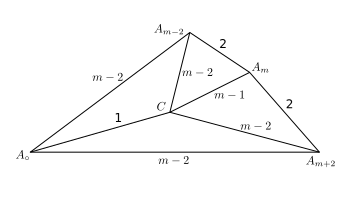
\includegraphics{vol32-figures/fig32-1.eps}}
\end{figure}

(In\pageoriginale the figure, the lengths of the paths are less than
or equal to the numbers marked along them.) 

\medskip
\noindent{\textbf{Case 2. {\boldmath$n$} odd.}
Let $n =2m+1$. Then $d(A_o, A_{m+1}) \leq m$. If
  $d(A_o, A_{m+1}) < m$, there is a path of length $< m$ from $A_o$
  to $A_{m+1}$, and we are through. If  $d(A_o, A_{m+1}) = m$, we
  proceed as in Case 1. See the figure below: 

\begin{figure}[H]
\centerline{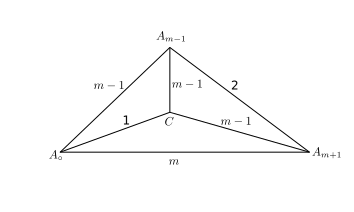
\includegraphics{vol32-figures/fig32-2.eps}}
\end{figure}

In the proof of Theorem \ref{chap3:thm3}, we shall use the following
lemma, a proof of which can be found in M. Eichler \cite{key1}, \S\ 12.  


\begin{lemma*}
  Suppose we are given, for each prime $p,a$ lattice $A_p$ in
  $\mathbb{Q}^n_p$ such that $A_p = E \otimes \mathbb{Z}_p$ except for
  finitely many $p$; here $E$ is the unit lattice in
  $\mathbb{Q}^n$. Then there exists a lattice $A$ in $\mathbb{Q}^n$ such
  that $A_p = A \otimes \mathbb{Z}_p$ for every $p$. (In fact $A =
  \bigcap \limits_p (\mathbb{Q}^n \cap A_p)$. 
\end{lemma*}

\setcounter{proofofThm}{2}
\begin{proofofThm}%%% 3
  Using Theorem \ref{chap3:thm2}, we shall now prove that $G = GL(n,
  \mathbb{Z}[P^{-1}])$ is finitely presentable, by induction on the
  cardinality of $P$. If $P = \phi , G = GL (n, \mathbb{Z})$, and this
  is finitely presentable (Remark following Lemma \ref{chap6:lem11},
  \ref{chap6}). Now 
  let $P \neq \phi$. We choose a $p \in P$, and consider $G$ as a group
  acting on the set $\mathcal{R}$ of lattices in $\mathbb{Q}^n_p$. The
  graph structure introduced on $\mathcal{R}$ is clearly invariant under
  the action of $G$; in fact the metric on $\mathcal{R}$ which defines
  its\pageoriginale graph structure is itself invariant under $G$. Further, it is
  clear that the isotropy group of $G$ at the unit lattice $E_p = E
  \otimes \mathbb{Z}_p$ of $\mathcal{R}$  is precisely $GL(n,
  \mathbb{Z}[P^{-1}_1])$, where $P_1 = P- \{p \}$. Hence if we verify
  that $G$ is transitive, then all the conditions of Theorem
  \ref{chap3:thm2} will be 
  satisfied on account of the induction hypothesis, and Theorem
  \ref{chap3:thm3} will 
  be proved. We shall now show that the subgroup $GL(n,
  \mathbb{Z}[P^{-1}_1])$ of $G$ is already transitive on $\mathcal{R}$. 
\end{proofofThm}

Given any $A \in \mathcal{R}$, consider the family $\{A_q,q \text{
  prime} \}$, where $A_q = E \otimes \mathbb{Z}_q$ for $q \neq p$, and
$A_{q} = A$. By the above lemma, there exists a lattice $A$ in
$\mathbb{Q}^n$ such that, for every prime $q,A_q = A \otimes
\mathbb{Z}_q$. Consider the $g \in GL(n, \mathbb{Q})$ such that
$g.E=A$. Then $g(E \otimes \mathbb{Z}_p)=A$ (where $g$ is now regarded 
as in $GL(n, \mathbb{Q}_p)$). But since, for every $q \neq p, g(E
\otimes \mathbb{Z}_q) = (E \otimes \mathbb{Z}_p)$, we must have $g \in
GL(n, \mathbb{Z}[p^{-1}])$, and our assertion is proved. 

\section{Groups generated by reflexions}\label{chap3:sec3}%sec 3

Let $M$ be a connected differentiable manifold. A diffeomorphism $r$
of $M$ onto itself is called a \textit{reflexion} if (i) $r^2 =$
identity, (ii) $M-M(r)$ is disconnected, where $M(r) =\{ x \in M| r(x)
=x \}$. Since, in a suitable coordinate neighbourhood of any $x \in M
(r)r$, acts as an orthogonal linear transformation (see Montogomery and
Zippin \cite{key1}, p.206), we see that $M-M(r)$ has exactly two connected
components which are carried each into the other by $r$, and that
$M(r)$ is a (not necessarily connected) submanifold of $M$ of
codimension one. 

\begin{thm}%the 4
  Let\pageoriginale $G$ be a discrete proper group of differentiable
  automorphisms of 
  a simply connected differentiable manifold $M$, generated by
  reflexions. Then $G$ has a presentation of the form $\{ r_{\alpha};
  (r_\alpha r_\beta)^{p_{\alpha \beta}} =e\}$, where the $r_\alpha$ are
  reflexions. 
\end{thm}

\begin{proof}
  Let $\mathcal{R}$ be the set of all reflexions belonging to $G$. Since
  $M(r))_{r \in \mathcal{R} }$ is a locally finite family, $M - \bigcup
  \limits_{r \in \mathcal{R}}M(r)$ is an open set; we denote the set of
  its connected components by $(W_i)_{ i \in I}$. $G$ acts on the set of
  $M(r)'s, r \in \mathcal{R};$ in fact $gM(r) = M(r^{g-1}), r^{g-1}=
  grg^{-1}$ being clearly a reflexion. Hence $G$ also acts on the
  $W'_i s$. 
\end{proof}

Let $W_o$ denote any one of the $W_i$. Let $\mathcal{R}' = \{ r \in
\mathcal{R}|$ there exists $x \in \bar{W}_o$ such that $r \in
\mathcal{R} \cap G(x)\}$. Let $\mathscr{L} (\mathcal{R}')$ be the free
group generated by $\mathcal{R}'$; we denote the natural injection
$\mathcal{R}' \to \mathscr{L}(\mathcal{R}')$ by $r \rightsquigarrow
r_L$. Let $K$ be the normal closure in $\mathscr{L}(\mathcal{R}')$ of
the set  
$$
\Bigg\{ (r_i)_L (r_j)^{\text{ ord } r_i r_j}_L | r_i, r_j \in
\mathbb{R}' , M(r_i) \cap M(r_i) \cap \bar{W}_o \neq \phi \Bigg\}. 
$$

We denote by $\varphi : \underbar{G} =\mathscr{L}(\mathcal{R}')/_{K}
\to G$ the natural homomorphism induced by $r_L \rightsquigarrow r$. 
Also, for any $r \in \mathbb{R}'$, we denote $r_L $ mod $K$ by
$\underbar{r}$. We shall prove by induction on the dimension of $X$
that  
\begin{enumerate}[(1)]
\item $\varphi : \underbar{G} \to G$ is a bijection
\item $G$ acts freely transitively on the set $(W_i)_{i \in I}$.
\end{enumerate}

For any $x \in M$ let $G_x$ (\resp $\underbar{G}_x$) be the subgroup of
$G$ (\resp $\underbar{G})$ generated by $\mathcal{R}' \cap
G(x)$ (\resp the $\underbar{r}$ such that $r \in \mathcal{R}' \cap
G(x))$.  

Since $G$ is discrete and proper, we have for every $x \in M$ a
coordinate neighbourhood\pageoriginale $V_x$ such that $V_x$ is $G(x)$-stable, and
$G(V_x|V_x) = G(x)$. We may assume the coordinate system so chosen
that $G(x)$ acts on $V_x$ by orthogonal linear transformations. We
assert that, for $x \in \bar{W}_o$, 
\begin{enumerate}[(a)]
\item $\varphi :\underbar{G}_x \to G_x$ is bijective,
\item for any $y \in V_x, G_y$ is simply transitive on the set of
  $W_i$ such that $y \in \bar{W}_i$, in particular, $G_x(\bar{W}_o
  \cap V) = V_x$. These assertions are easy to verify if $\dim X \leq
  2$; if $\dim X \geq 3$, they follow from the induction hypothesis
  (1) and (2), when we consider the action of $G_x$ on the spheres
  about $x$ in $V_x$. 
\end{enumerate}

Now let $Y$ be the quotient space of $\underbar{G} \times
\bar{W}_o(\underbar{G}$ having the discrete topology) by the
equivalence relation 
$$
(t',x') \sim (t,x) \Longleftrightarrow x' =x \text{~ and~ } t^{-1}t \in
  \underbar{G}_x. 
$$

The mapping $(t,x) \rightsquigarrow \varphi (t) x$ of $\underbar{G}
\times \bar{W}_o$ to $M$ induces a mapping $f:Y \to M$. Similarly the
action $(t,x) \rightsquigarrow (st,x)$ of $\underbar{G}$ $G
\times \bar{W}_o$ induces an action of $\underbar{G}$ on
$Y$. $\underbar{G}$ acts on $X$ through $\varphi$. It is clear that
$f$ commutes with the action of $\underbar{G}$. We proceed to show
that $f:Y \to M$ is a connected covering. 
\begin{enumerate}[(i)]
\item \textit{$Y$ is connected}. This is clear since for every $r \in
  \mathcal{R}', \underbar{r}\, q (e \bar{w}_\circ)\cap q (q,
  \bar{W})\circ) \neq \phi$. Here $q :
  \underbar{G} \times \bar{W}_o \to Y$ is the natural map. 
\item \textit{ $f$ is locally injective }. It is sufficient to know
  that\pageoriginale $f$ is injective in a neighbourhood of any $q(e, x),x \in
  \bar{W}_o$. Now $\underbar{G}_x \times (V_x \cap \bar{W}_o)$ is
  saturated with respect to $q$, hence $q (\underbar{G}_x \times (V_x
  \cap \bar{W}_o))$ is a neighbourhood of $q(e,x)$. Using the
  inductive assertions a) and b), we see that $f$  is injective
  on $ q (\underbar{G}_x \times (V_x \cap \bar{W}_o)$. 
\item \textit{$f$ is surjective}. We must show that  $\varphi
  (\underbar{G}) \bar{W}_o =M$. Now, $\varphi (\underbar{G})
  \bar{W}_o$ is obviously closed in $M$, being a locally finite union
  of closed sets. But it is also open, since for any  $ x \in
  \bar{W}_o ,\varphi (\underbar{G}_x) \bar{W}_o = G_x \bar{W}_o$ is a
  neighbourhood of $x$ by the inductive assertion $b$). 
\item \textit{$f$ has local sections}. Since $f$  commutes with the
  action of $\underbar{G}$, and $\phi (\underbar{G}) \bar{W}_o =M$, it is
  sufficient to consider points of $\bar{W}_o$. 

Now let $N$ be the subgroup of $\underbar{G}$ defined by 
$$
N =\{ n \in \underbar{G}| \varphi(n) \bar{W}_o = \bar{W}_o \}.
$$
Clearly $N \supset $ker $\varphi$. For $n \in N$ and $r \in
\mathcal{R}'$, it is clear that $r^n(=r^{\varphi(n)}) \in
\mathcal{R}'$.  Further if $r,r' in \mathcal{R}'$ and $M(r) \cap M(r')
\cap \bar{W}_o \neq \phi$, we have also $M(r^n) \cap M(r'^n) \cap
\bar{W}_o \neq \phi$. Hence we can define the automorphism $h
\rightsquigarrow h^n$ of $\underbar{G}$ by setting $(\underbar{r})^n =
\overline{(r^n)}$. Clearly $\varphi(h^n) = \varphi(n^{-1}) \varphi(h)
\varphi(n)$. 

Now, for any $n \in N$ and any $x \in \bar{W}_o$, we define the
section $\sigma_n: V_x \to Y$ of $f$ by  
$$
\sigma_n(\varphi(t)y) = q(n t^n,\varphi(n^{-1})y); t \in
\underbar{G}_x, y \in V_x \cap \bar{W}_o. 
$$
By (ii), $\sigma_n$ is well-defined.
\item \textit{$f^{-1} (V_x) = \bigcup \limits_{n \in N} \sigma_n
  (V_x)$.} Let $h \in \underbar{G}, z \in \bar{W}_o$, and let
  $f(q(h,z)) \in V_x$. Then $\varphi(h) = \varphi(t)y$, with $t \in
  \bar{G}_x$, and $y \in V_x \cap \bar{W}_o$; thus $\varphi(h^{-1} t)
  y =z$. Now, since $\underbar{G}_z$ is transitive on the $\bar{W_i}$
  containing\pageoriginale $z$, there exists $s \in \underline{G}_z$ such that
  $s^{-1} h^{-1} t \in N$. Let $n = t^{-1}$hs. Then  
$$
q(tn, \varphi(n^{-1})y)  = q(h,z).
$$

Now, Since $\varphi(t ~n)= \varphi(n~ t^n)$, there exists $u \in \ker
\varphi$ such that $tn= unt^n= unt^{un}$. Then  
\begin{align*}
  q(h, z) &= q( tn, \varphi (n^{-1}) y)\\
  &=q(unt^{un}, \varphi ((un)^{-1})) y\\
  &= \sigma_{un}(\varphi (t) y),
\end{align*}
and (V) is proved.

\item  For $n,n' \in N , \sigma_n (V_x) \cap \sigma_{n'} (V_x) \neq
  \phi \Rightarrow n=n'$. Let $n, m \in  N, \sigma_n (y)=
    \sigma_m(y)$ for some $y \in V_x$. Since $f$ is locally injective,
    and $G_x W_o$ is dense in $V_x$, there $z \in V_x \cap G_x W_o$
    such that $\sigma_n (z) = \sigma_m (z)$. Let $z =\varphi(t) z' , t
    \in \underline{G}_x$ and $z' \in W_o \cap V_x. \sigma_n (z)=
    \sigma_m (z)$ gives  
$$
\varphi (n^{-1}){z'} = \varphi(m^{-1}){z'} \Rightarrow \varphi(nm^{-1})
\in G(z') \subset G(x), 
$$
and $(nt^n)^{-1}(mt^m) \in \underline{G}_{z'} =e$. 

Hence $n^{-1}m =t^n(t^{-1})^m$. Now $t^n \in
\underline{G}_{\varphi(n^{-1})x}$ and $t^m \in G_{\varphi(m^{-1})x'}$
since $t \in \underline{G}_x$. But, since $\varphi(nm^{-1}) \in G(x),
\varphi(n^{-1})x= \varphi(m^{-1}) x$, hence $n^{-1} m \in
\underline{G}_{\varphi(n^{-1})x}$. Since $n^{-1} m \in N$, it follows
by the induction assumption b) that $n^{-1}m =e$, and (vi) is
proved. 
\end{enumerate}

Thus\pageoriginale $f: Y \to M$ is a connected covering. Since $M$ is simply
connected, $f$ is bijective. Since the fibres of $f$ are parametrised
by $N \supset \ker \varphi, \varphi$ is injective. And then $N= \{e\}$
means precisely that $\varphi(\underline{G})$ is simply transitive on
the $W_i$. It follows easily that for every $r \in \mathscr{R}$, there
exist $h \in \varphi(\underline{G})$ and $r' \in \mathscr{R'}$ such
that $r' = r^h$; hence $\varphi (\underline{G})= G$, and the
assertions (1) and (2) are proved. 
